In master-slave cluster, a node is either a \textbf{master} or a \textbf{slave}. There is one and only one master in a cluster; master has no master to itself but slaves always have either a master or another slave as its master. Together all these nodes forms a tree-like topology with the root of the tree being the master of the cluster. 

In this mode each node has a sidecar service to assist master-slave replication.  Upon initiation, slaves post a request to its master's sidecar service to register as a known slave.

Masters and slaves handles subscribe action just as single machine implementation. Therefore, the system could easily increase reading throughput linearly by adding more nodes into the cluster. 

For publish, a slave would propagate the message to its master until the master of the cluster. Once received the message, the master would broadcast the message to all its slaves through their master-slave sidecar service, and then perform a publish action to its subscribers same as single-machine service. For slaves, they each manages a thread to listen to confirmed publish messages from its master, publish the message to its subscribers, and keep relaying the message to its slaves.

Since master-slave cluster forms a tree, one of the proposed design is to let nodes reserve a special topic for its slaves, and the slaves can just subscribe to the special topic to relay messages to their subscribers. However, the implementation is not adapted eventually for two reasons: first, developers have to introduce a guarding scheme to prevent users from interrupting system messages in reserved topics; second, the messages in reserved topic will have to be serialized at master to include metadata such as topic name and then deserialized at slaves, which introduces unnecessary operations. 

\begin{figure}[H]
	\centering
	\begin{tikzpicture}[shorten >=1pt,node distance=2cm,on grid,auto]
		\node[state] (0) {master};
		\node[state] (1) [below left=of 0]{slave-0};
		\node[state] (2) [below right=of 0]{slave-1};
		\node[state] (3) [below=of 1]{slave-2};
		\path[->]
			(1) edge node {} (0)
			(2) edge node {} (0)
			(3) edge node {} (1);
	\end{tikzpicture}
	\caption{Master-Slave Cluster Topology}
\end{figure}
	
The researchers set up a cluster with 4 nodes organized as figure 3 for load testing. This organization includes all potential master-slave relation that could exists in master-slave mode, which could provide a more comprehensive demonstration of cluster performance.
	
\begin{figure}[H]
	\centering
	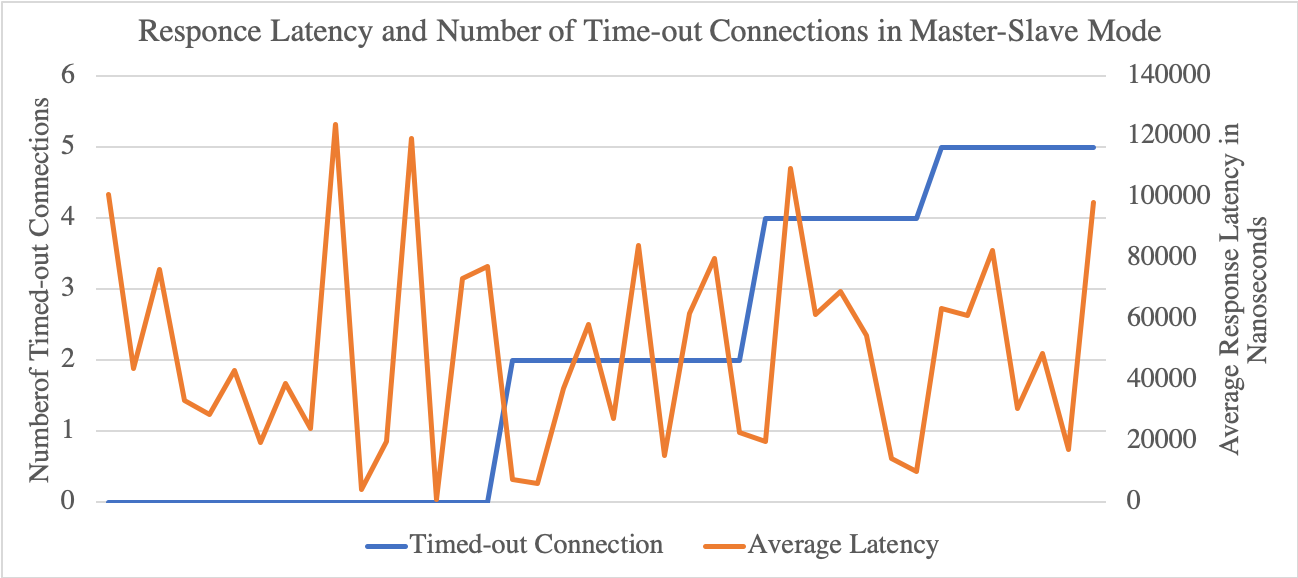
\includegraphics[scale=0.33]{figure/master-slave/performance.png}
	\caption{Master-Slave Performance}
\end{figure}

\begin{figure}[H]
	\centering
	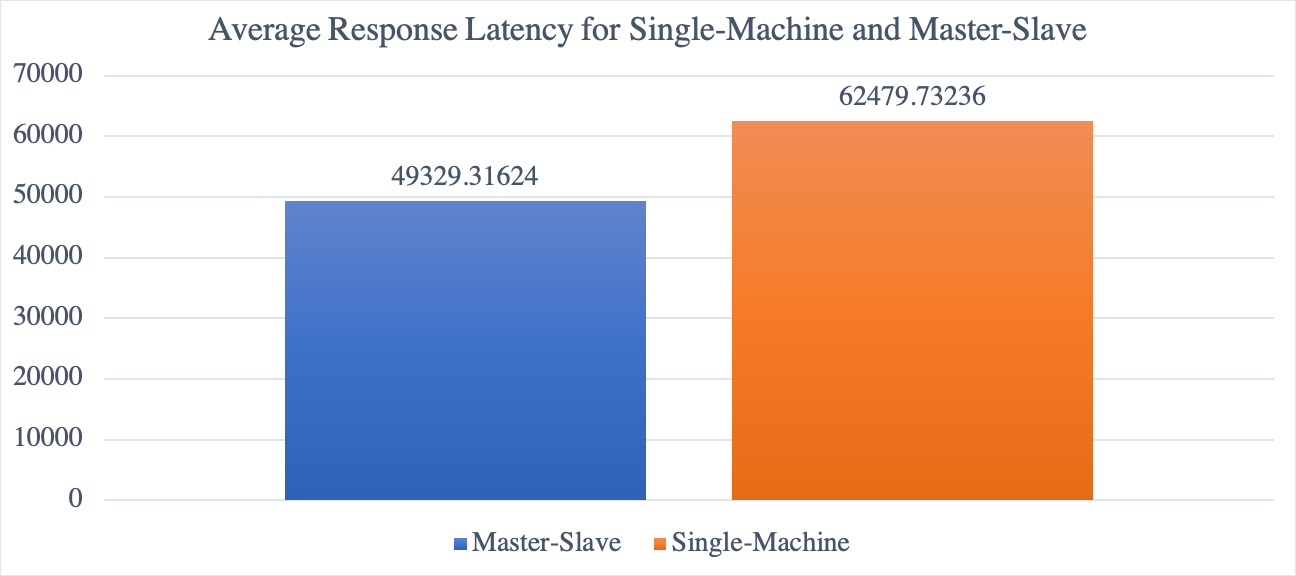
\includegraphics[scale=0.33]{figure/master-slave/response-latency.png}
	\caption{Single-Machine/Master-Slave average response latency}
\end{figure}

Figure 4 and 5 provide an overview of the capacity of master-slave Pub/Sub cluster. The statistics reflects here that, comparing to single-machine implementation, master-slave is slightly faster and has fewer timed out connections throughout the testing process. The testing program evenly distributed clients among nodes in the cluster, therefore causing each node  to handle only a quarter of load using the same amount of resources as the single-machine instance. The researchers actually expected master-slave architecture to be slower due to potential latency that may caused by message propagation through network. But since the testing cluster is hosted as containers sharing a virtual network on a single machine, the effect of network latency appears to become negligible. This finding could be helpful to users when they apply Pub/Sub in production, as they might be able to use master-slave mode to dispatch or collect data rapidly across regions with the leverage of reliable and performant network service, such as Google Could's high-performance premium tier network solution\citep{google-cloud-network}.

Master-slave's demonstrate decent potential, but its performance is in trade of reliability. If one node were to go down, all of the node's slaves and sub-slaves will lost sync with the rest the cluster at the same time. Besides, a master-slave cluster's performance is strongly correlated to its topology. If the cluster tree is too deep, or some of the nodes serving too many clients, the cluster's performance could be significantly affected. Only a balanced-tree of reasonable height with clients evenly distributed among nodes would make the cluster perform the finest. 
